% Falar que o Brasil é Continental
% Falar sobre a base
% Publico destinado.

O Brasil é um país gigante por natureza. Segundo dados do IBGE (2021), o Brasil é o quinto maior país em extensão territorial. Nosso país é formado por 8.515.767 km$^2$, perdendo apenas para Rússia, Canadá, China e Estados Unidos. Se considerarmos o aspecto populacional, o Brasil também se destaca. Atualmente o Brasil possui a sexta maior população, com mais de 210 milhões de pessoas \cite{ibge2021}. Devido as características territoriais e populacionais, o Brasil possui um grande histórico de acidentes ambientais. Por este motivo, desde 2014, o Instituto Brasileiro do Meio Ambiente e dos Recursos Naturais Renováveis (IBAMA) mantém o Sistema Nacional de Emergências Ambientais (SIEMA), uma base de dados com os acidentes ambientais mapeados deste século \cite{ibama2021}. Diante deste cenário, esta dissertação visa apresentar informações relevantes sobre os acidentes ambientais registrados no Brasil, com o objetivo de conscientizar adultos sobre a importância de denunciar este tipo de ocorrência.

% Falar sobre os incidentes

A base de dados do SIEMA, até o dia 16 de Outubro de 2021, era composta de 12.005 registros. Esta base contém acidentes ambientes das mais diversas proporções, que vão desde eventos não noticiados na grande mídia, até acidentes catastróficos, como o rompimento da barragem de Mariana, em 2015 \cite{wanderley2016desastre}. Analisando os dados, é possível observar que mesmo sendo uma das menores regiões em território, pouco menos de 11\%, o Sudeste se destaca com mais de 63\% dos acidentes ambientais registrados. O Sul, menor região do Brasil em extensão territorial (menos de 7\%) aparece em segundo, com 12,5\% dos acidentes registrado. Nordeste com 9,8\%, Centro-Oeste com 6\% e a Região Norte com 4,3\% completam a lista do acidentes ambientais mapeados pelo SIEMA. Outros 4,3\% das ocorrências na base não apresentam informações de onde ocorreram. Se considerarmos todos os estados brasileiros, Minas Gerais é o principal foco de desastres ambientais, com mais de 25\% das ocorrências. A Figura \ref{fig:ocorrencias} apresenta as ocorrências distribuídas no mapa do território brasileiro.

\begin{figure}[!h]
    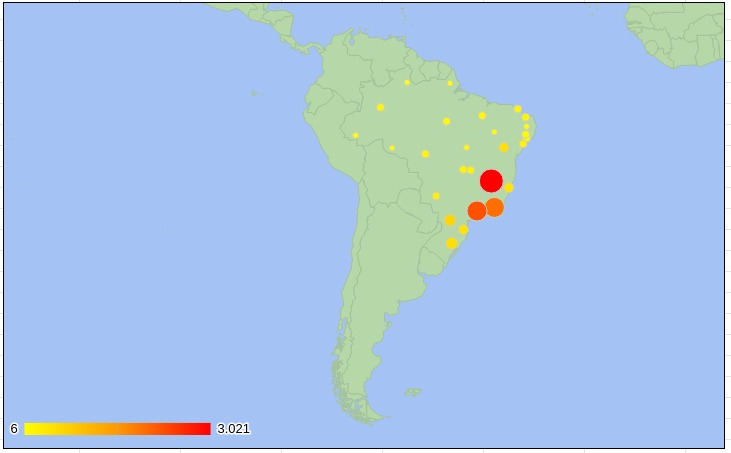
\includegraphics[scale=0.45]{fig/mapa_ocorrencias.jpeg}
    \centering
    \caption{Acidentes ambientais registrados no Brasil neste século.}
    \label{fig:ocorrencias}
\end{figure}

% Falar sobre a natureza dos incidentes/impacto

A base de dados também apresenta uma informação importante, que é a origem do acidente ambiental. Analisando os dados, podemos observar que aproximadamente 32\% das ocorrências (3929 eventos) se originam por meio de algum acidente rodoviário. O Brasil possui uma das maiores malhas rodoviárias do planeta e, segundo a Confederação Nacional do Transporte (CNT), apenas 12,4\% desta malha é pavimentada. A malha rodoviária brasileira, no geral, é de baixa qualidade de infraestrutura e, mesmo assim, movimenta mais de 60\% das mercadorias e mais de 90\% dos passageiros em território nacional. Em 2017, somente nas rodovias federais, foram registrados quase 60 mil acidentes com vítimas, e mais 6.200 óbitos \cite{cnt2021}. Por este motivo, redobre a atenção ao volante. Vidas estão em jogo e desastres ambientais também. A Figura \ref{fig:origens} apresenta a distribuição dos acidentes ambientais registrados conforme sua origem.

\begin{figure}[!h]
    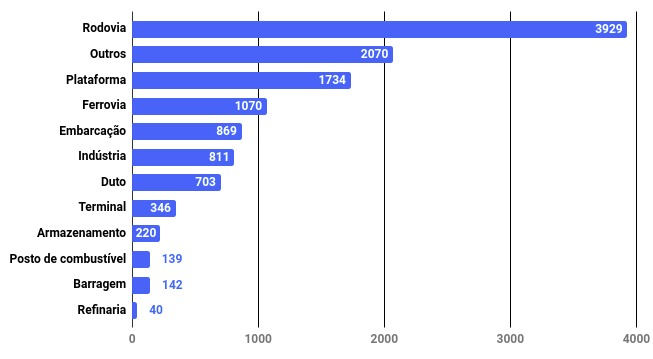
\includegraphics[scale=0.55]{fig/origens.jpeg}
    \centering
    \caption{Distribuição dos acidentes ambientais registrados conforme origem.}
    \label{fig:origens}
\end{figure}

%\begin{figure}[h]
%    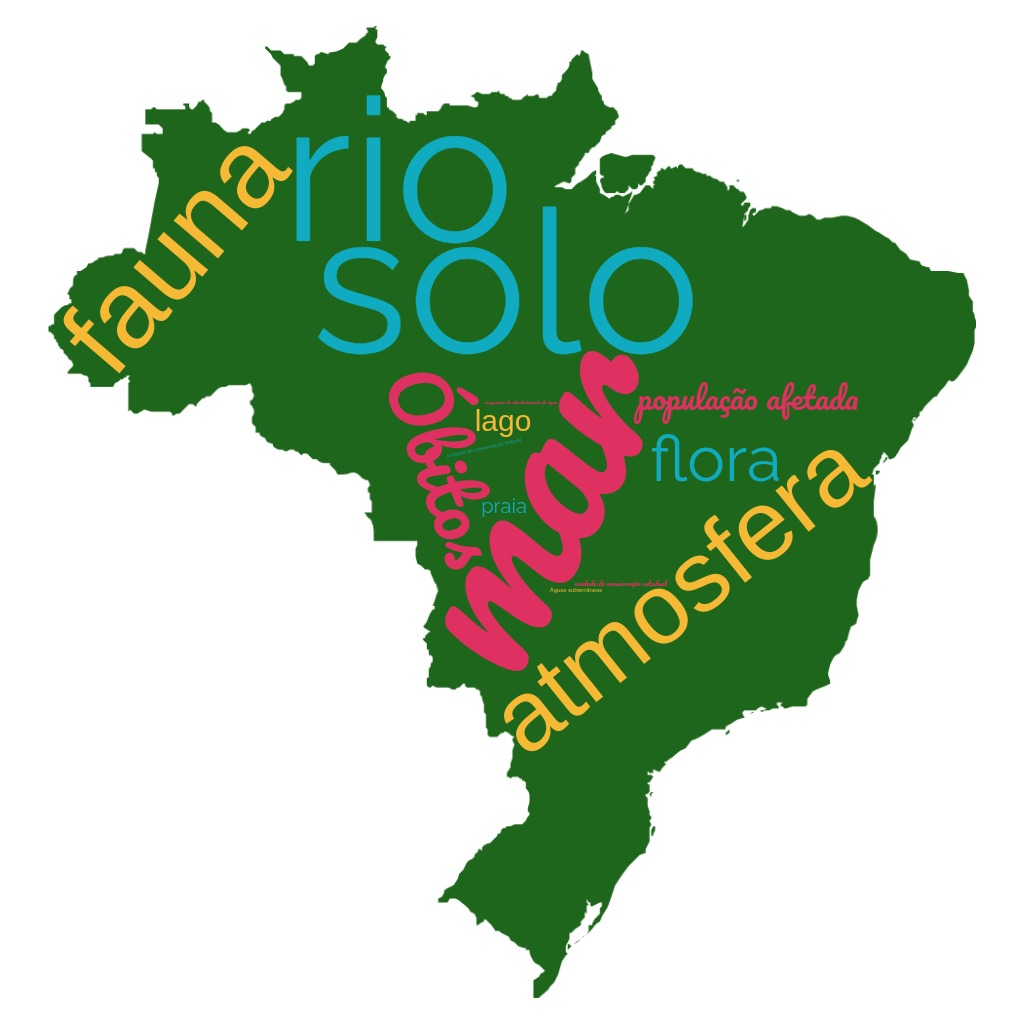
\includegraphics[scale=0.25]{fig/danos.jpg}
%    \centering
%    \caption{Distribuição das ocorrências no Brasil.}
%    \label{fig:danos}
%\end{figure}

% Falar sobre quem atua - herois

Grande parte dos acidentes ambientais (quase 4 mil ocorrências) despejam líquidos tóxicos e corrosivos. Estes eventos degradam nossa fauna, flora, além de matar nossos rios, mares e nosso solo. Muitas instituições lutam constante e incansavelmente contra esses acidentes ambientes. Dos 12.005 eventos catálogos, 14,8\% tiveram atuações do Corpo de Bombeiros. Vale destacar também a participação das Polícias Civil, Rodoviária e Militar, que atuaram em 12\% das ocorrências. O IBAMA e os órgãos estaduais/municipais de Meio Ambiente também atuaram aproximadamente em 10\% dos eventos. Por fim, vale mencionar também a atuação de outras instituições contra acidentes ambientais, que totalizam 63,3\% dos registros. Por este motivo, ao ver qualquer acidente ambiental, relate imediatamente a alguma autoridade. A Figura \ref{fig:quematua} apresenta a distribuição das instituições que atuam contra acidentes ambientais no Brasil.

\begin{figure}[!h]
    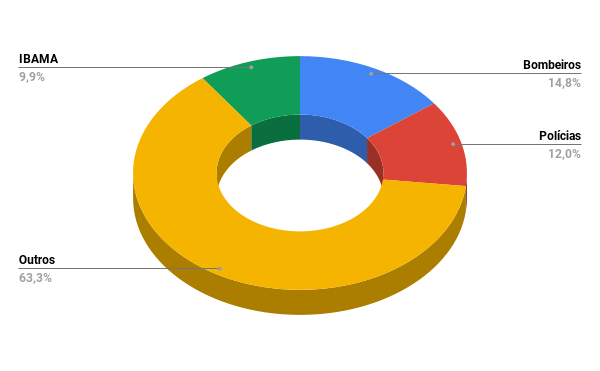
\includegraphics[scale=0.6]{fig/quematua.png}
    \centering
    \caption{Instituições que atuam contra acidentes ambientais no Brasil.}
    \label{fig:quematua}
\end{figure}

% Falar sobre conscientização
% Concluir

Cuidar do meio ambiente é garantir que as gerações futuras terão o que usufruir. A população global vem crescendo vertiginosamente, e somente a Educação Ambiental \cite{reigota2017educaccao} e conscientização podem garantir que a natureza não entre em colapso em breve. Infelizmente, observando os dados, podemos perceber que muitos dos acidentes ambientais não possuem todos os dados registrados. Por este motivo, leiam sobre o assunto, eduquem os mais jovens, denunciem os acidentes ambientais, e até mesmo as atitudes suspeitas para evitar que estes eventos aconteçam. Cuidar do meio ambiente é obrigação de todos. A natureza agradece.

